\Chapter{Resultados e discussões}

Um sistema, cujo objetivo principal era implementar um forma de interação homem-máquina de forma não convencional através de reconhecimento de gestos por visão computacional, foi implementado neste trabalho. O modelo é testado utilizando-se cinco vídeos gravados de cada um dos gestos isolados, outros vídeos foram gravados onde os mesmos gestos apresentavam-se de forma contínua e por último um vídeo longo onde todos os gestos são realizados intercalados de forma contínua sem ordem prevista. Um vídeo de outro usuário executando os gestos também foi gravado com a finalidade de testar os resultados do aplicativo.

Como visto anteriormente, um avatar foi desenvolvido para que técnicas de visão computacional pudessem ser utilizadas em conjunto com modelos ocultos de Markov com o objetivo de enviar comandos de controle para esse avatar atuar no ambiente virtual.


\section{A aplicação em interação com objetos virtuais}

Os módulos de vídeos e ambiente virtual são inicializados ao mesmo tempo, então a captura de cada frame do vídeo é iniciada. O avatar fica realizando a animação padrão, enquanto o módulo de identificação reconhece o gesto realizado no último segundo.

As Figuras \ref{img:sistema_1}, \ref{img:sistema_2}, \ref{img:sistema_3} e \ref{img:sistema_4} exibem imagens do sistema reconhecendo os gestos corretamente e o avatar realizando as animações equivalentes. A Figura \ref{img:sistema_krishynan} demonstra um outro usuário utilizando o sistema, mas não tendo participado do processo de treinamento, ou seja, um usuário B utilizou o mesmo módulo de treino que foi alimentado com vídeos do usuário A.

\begin{figure}[!htbp]
  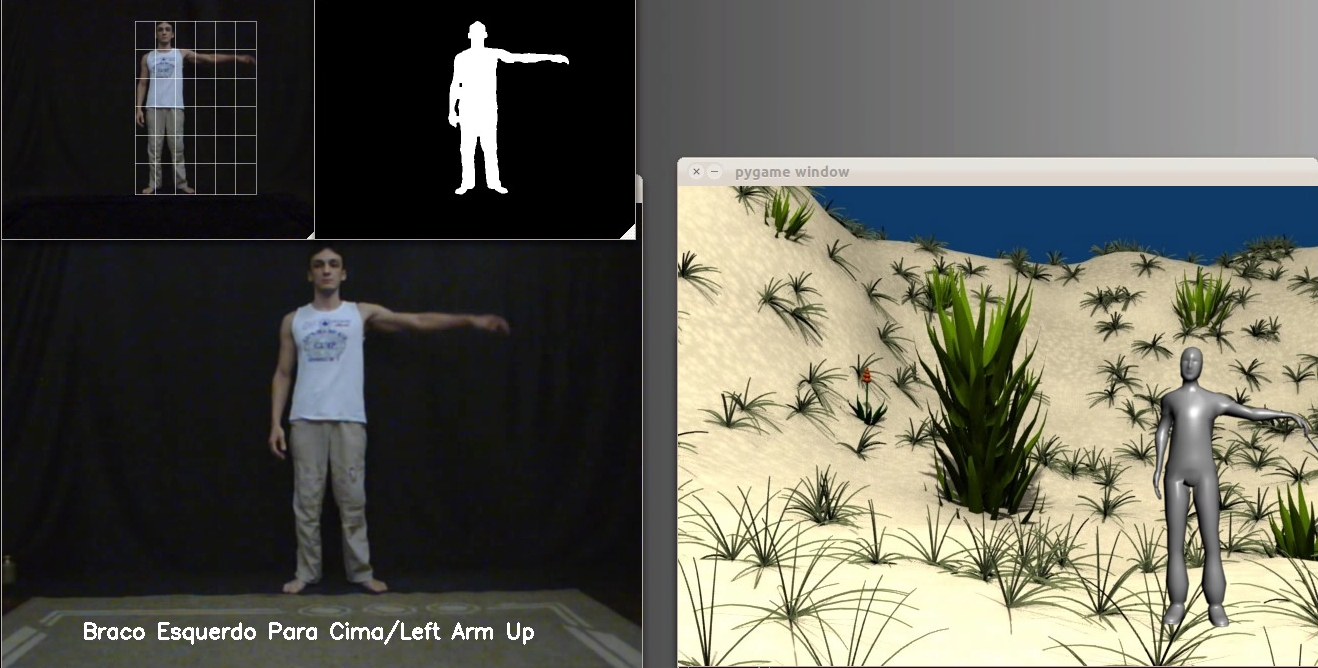
\includegraphics[scale=0.35]{imagens/sistema_1.jpg}
  \caption{Situação de reconhecimento do gesto levantar o braço esquerdo no sistema.}
  \label{img:sistema_1}
\end{figure}

\begin{figure}[!htbp]
  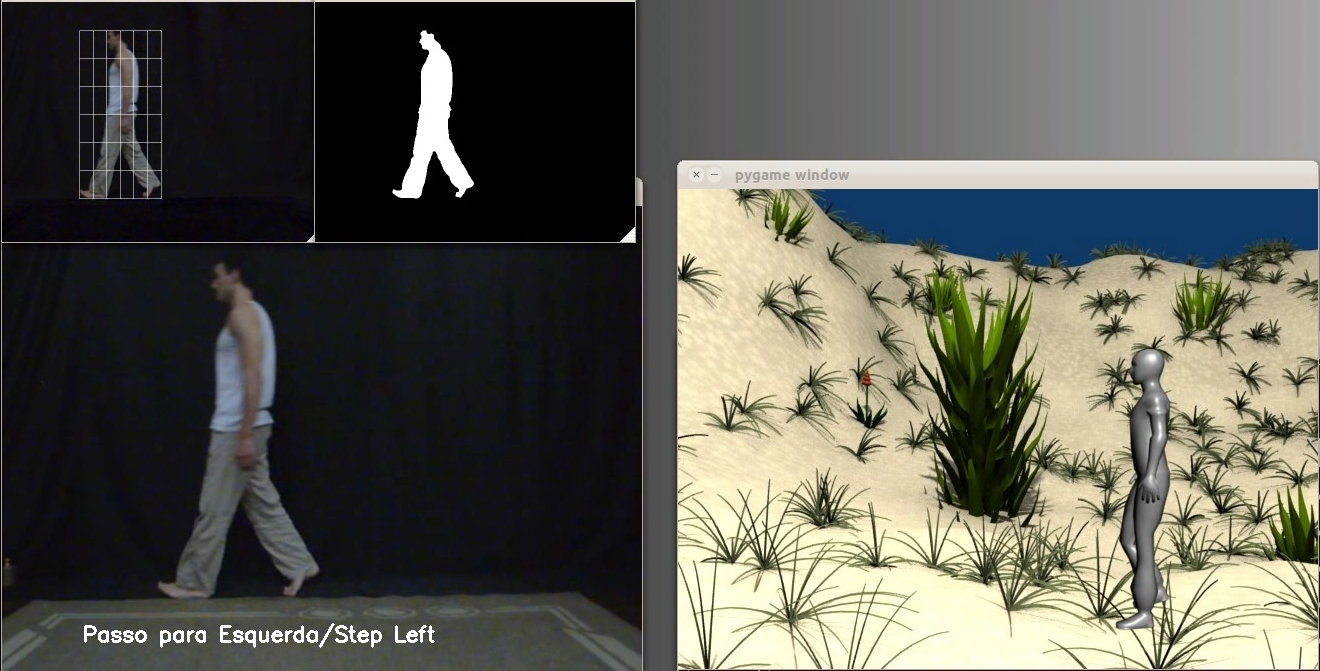
\includegraphics[scale=0.35]{imagens/sistema_2.jpg}
  \caption{Situação de reconhecimento do gesto passo para esquerda no sistema.}
  \label{img:sistema_2}
\end{figure}

\begin{figure}[!htbp]
  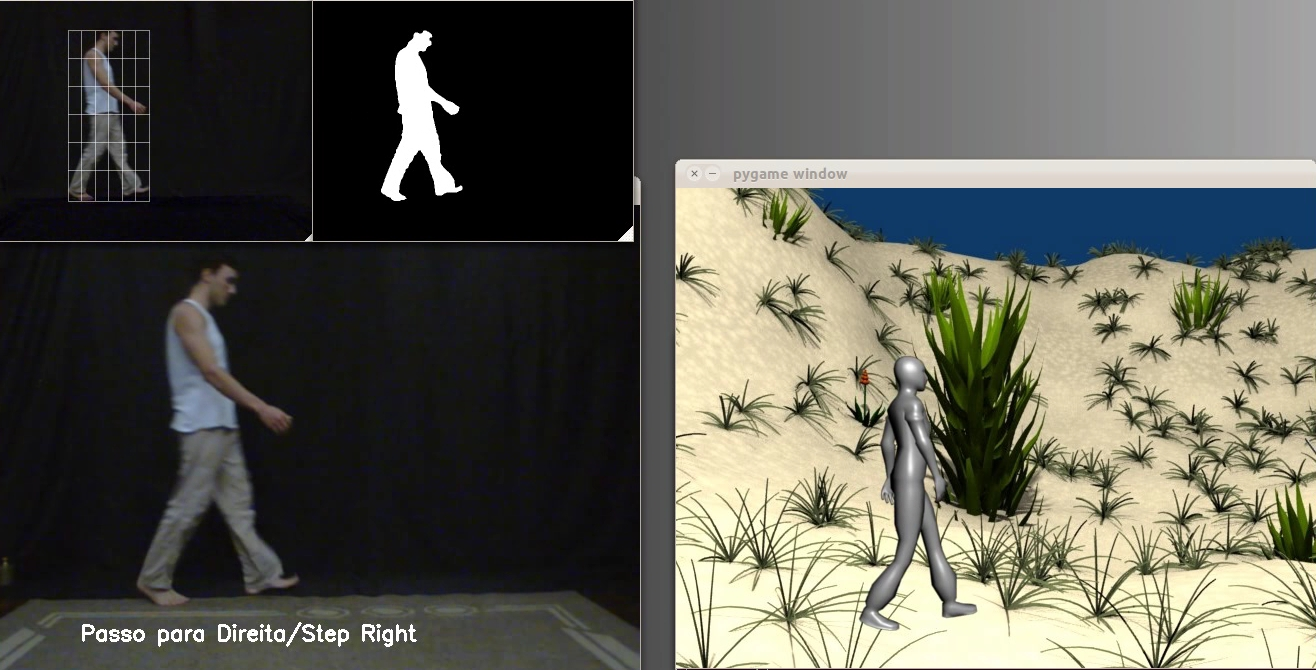
\includegraphics[scale=0.35]{imagens/sistema_3.jpg}
  \caption{Situação de reconhecimento do gesto passo para direita no sistema.}
  \label{img:sistema_3}
\end{figure}

\begin{figure}[!htbp]
  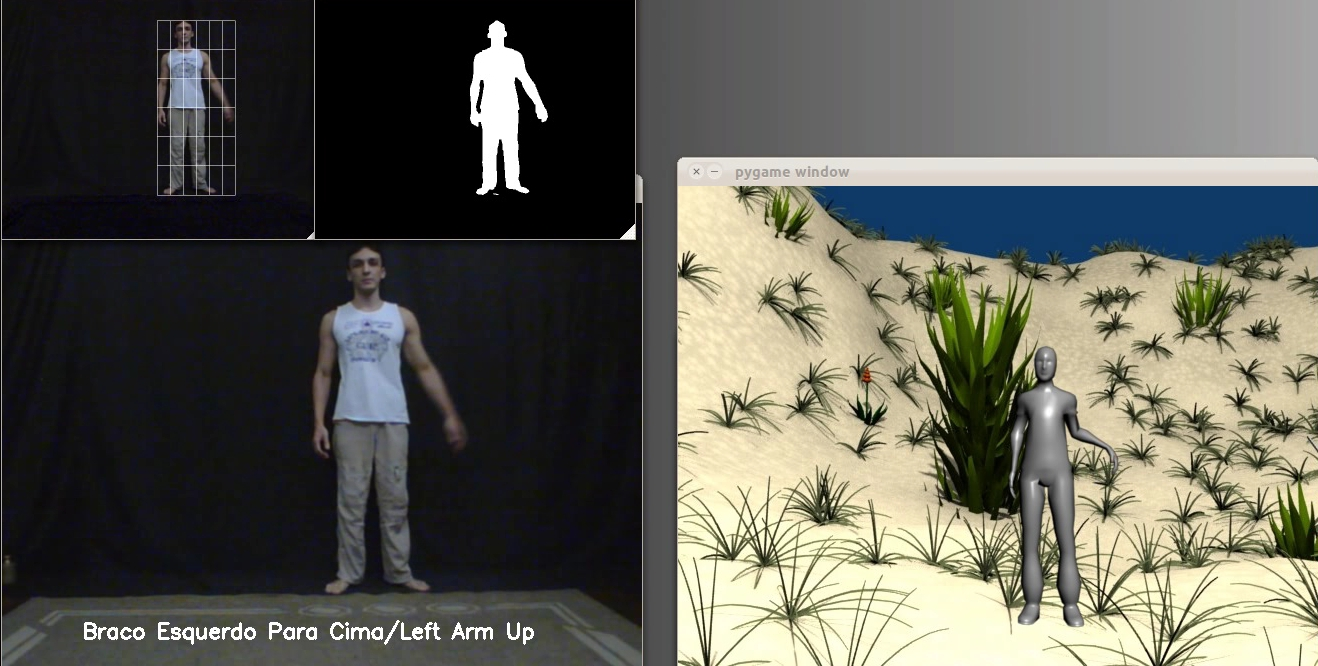
\includegraphics[scale=0.35]{imagens/sistema_4.jpg}
  \caption{Outra situação de reconhecimento do gesto levantar o braço esquerdo no sistema.}
  \label{img:sistema_4}
\end{figure}

\begin{figure}[!htbp]
  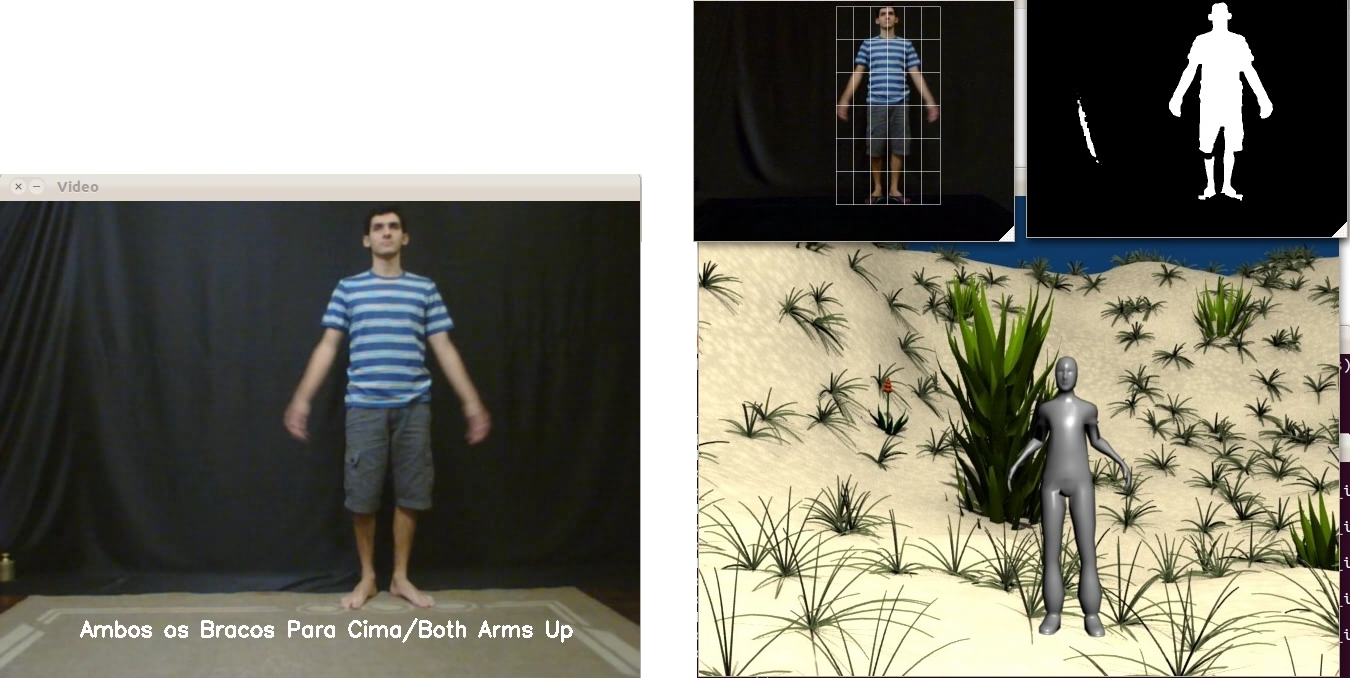
\includegraphics[scale=0.35]{imagens/sistema_krishynan.jpg}
  \caption{Usuário B testando o sistema treinado pelo usuário A.}
  \label{img:sistema_krishynan}
\end{figure}

O sistema não se comportou de forma esperada quando um gesto de andar para direita ou para esquerda acontecia seguido da postura parado de frente para a câmera. Isso aconteceu principalmente porque os vídeos que treinaram o sistema não continham um exemplo desse gesto, em outras palavras, as HMMs treinadas para reconhecerem os gestos de passos, nunca começavam com o símbolo 0, que é a codeword para a postura parado de frente, então o gesto de caminhar só era reconhecido se o usuário já estivesse de lado no ínicio das sequências desses gestos. A Figura \ref{img:andar_from_parado} ilustra o gesto acima descrito.

\begin{figure}[!htbp]
  \centering
  \subfigure{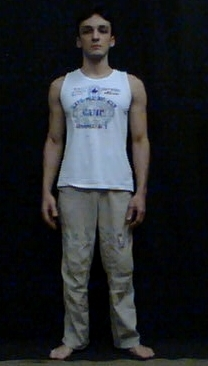
\includegraphics[scale=0.35]{imagens/andar_from_parado_1.jpg}}
  \subfigure{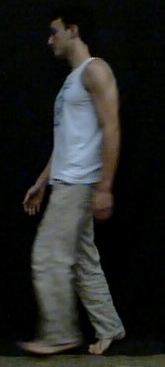
\includegraphics[scale=0.35]{imagens/andar_from_parado_2.jpg}}
  \subfigure{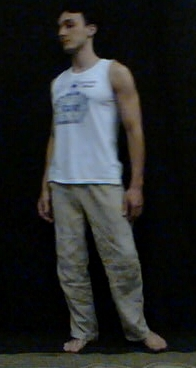
\includegraphics[scale=0.35]{imagens/andar_from_parado_3.jpg}}
  \subfigure{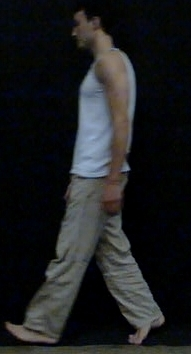
\includegraphics[scale=0.36]{imagens/andar_from_parado_4.jpg}}
  \caption{Gesto não reconhecido nos primeiros testes do sistema.}
  \label{img:andar_from_parado}
\end{figure}


Essa situação foi resolvida, injetando alguns símbolos 0 nas sequências de treinos dessas HMMs. As Figuras \ref{img:HMM_1_apos_treino_2} e \ref{img:HMM_2_apos_treino_2} apresentam os grafos dessas novas HMMs.

\begin{figure}[!htbp]
  \center
  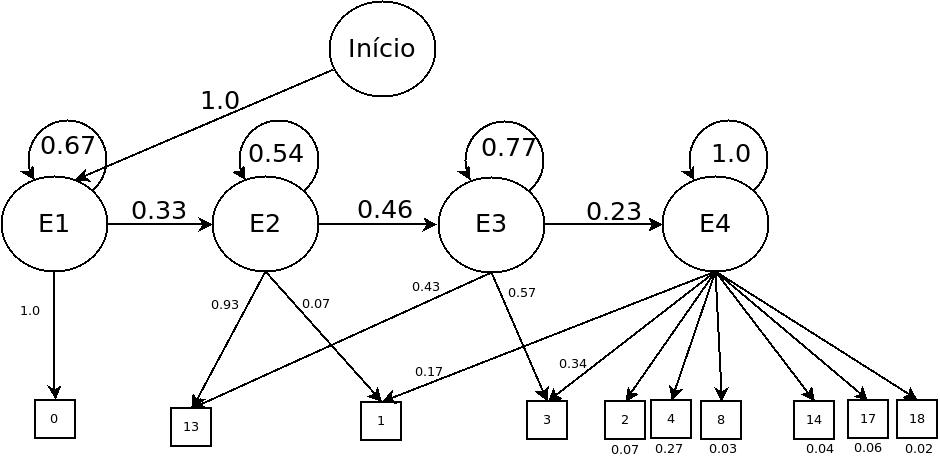
\includegraphics[scale=0.35]{imagens/HMM_1_apos_treino_2.jpg}
  \caption{Parâmetros da HMM treinada com os vídeos do gesto passo para direita após a injeção de símbolos 0.}
  \label{img:HMM_1_apos_treino_2}
\end{figure}

\begin{figure}[!htbp]
  \center
  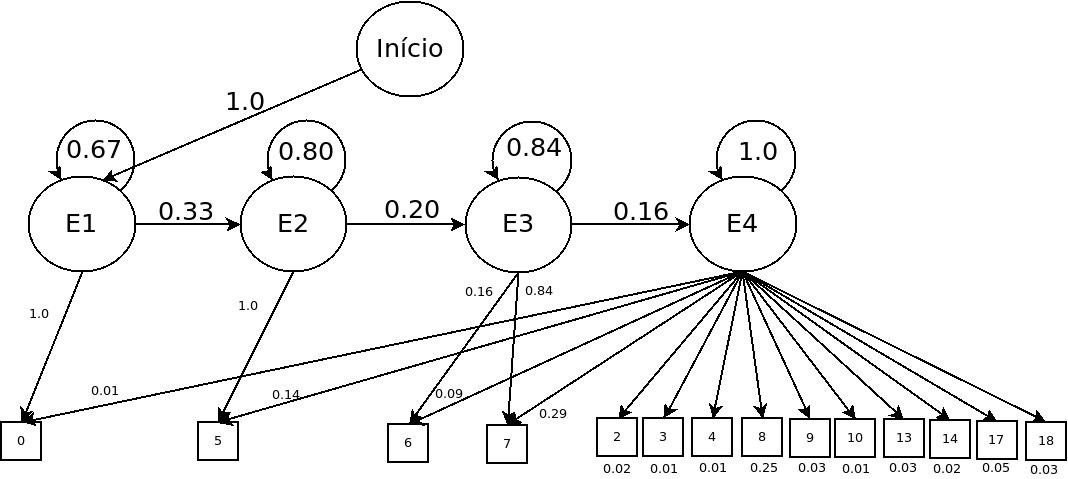
\includegraphics[scale=0.35]{imagens/HMM_2_apos_treino_2.jpg}
  \caption{Parâmetros da HMM treinada com os vídeos do gesto passo para esquerda após a injeção de símbolos 0.}
  \label{img:HMM_2_apos_treino_2}
\end{figure}

Essas HMMs reconhecem com sucesso os gestos anteriormente descritos, porém os gestos que eram reconhecidos antes agora não são reconhecidos, porque essas HMM só reconhecem os gestos de caminhar se as sequências forem inicializadas com o símbolo 0.

Esse problema foi resolvido alterando no processo de modelagem dessas duas HMMs, os parâmetros do vetor \(\pi\), que passaram a assumir valores com probabilidades iguais de começar em qualquer um dos quatro estados
\[
 \pi =
 \begin{pmatrix}
  0.25 & 0.25 & 0.25 & 0.25
 \end{pmatrix}.
\]

A topologia dessas HMM também foi alterada para o modelo totalmente conectado, isso resolveu o problema de forma que o gesto, além de poder começar em qualquer um dos estados, todos os estados poderiam retornar as quatro codewords de seus gestos. Agora o gesto de andar para direita, por exemplo, poderia começar pelas codewords 0, 1, 2, 3 ou 4 e todas esses símbolos poderiam aparecer em qualquer ordem que a sequência ainda seria reconhecida.

Se o interesse fosse manter a topologia \textit{Left Right Banded}, devido a sua taxa melhor de detecção segundo os trabalhos anteriormente comentados, seria preciso criar duas HMMs para cada gesto de caminhar.
 Um para a situação onde o usuário já se encontra de lado e outra para a situação onde o usuário se encontra virado de frente para a câmera. Essa situação também poderia ser resolvida, fazendo-se pequenas alterações na HMM treinada para que no seu primeiro estado ela possa retornar tanto o símbolo 1 quanto o símbolo 0. Avaliar se essas soluções apresentarão melhores probabilidades nos reconhecimentos é um dos motivos para trabalhos futuros.

Outro problema encontrado é quando o usuário fica parado em frente a câmera sem executar gesto algum, haverá uma sequência contendo apenas símbolos 0 nesse caso, se um pequeno ruído entrar nessa sequência, por exemplo, um simbolo de algum gesto de levantar o braço, uma das HMM vai retornar uma probabilidade mesmo que muito baixa, daquele gesto ter acontecido e ele na verdade não aconteceu. Seria preciso criar uma HMM para a situação do usuário ficar parado na maior parte do tempo ou definir uma tolerância nas probabilidades, para que quando uma probabilidade for muito baixa esse gesto não seja enviado para o módulo do ambiente virtual. Avaliar essas soluções e decidir qual seria melhor, também é motivo para trabalhos futuros.

Mesmo considerando esses problemas, o desempenho do sistema é muito satisfatório.

